\subsection{Estudo do espaço de trabalho do manipulador}

Para uma avaliação técnica das soluções, é necessária a análise do espaço de
trabalho, assim como a assegurar uma alta manipulabilidade em toda a trajetória
a ser traçada. A escolha de um manipulador industrial, no contexto da aplicação
desejada, é um compromisso entre o tamanho do manipulador e o espaço disponível.
Um manipulador de grande porte garante que todos os pontos a serem metalizados
sejam alcançados sem problemas, entretanto pode tornar inviável que o mesmo se
movimente no espaço confinado e consiga passar pelos acessos da turbina. Por
esse motivo, é necessário que a escolha do manipulador seja ótima no aspecto do
tamanho do manipulador e de seus graus de liberdade, para que seja possível
se especificar o menor manipulador possível que atenda com uma certa margem de
segurança a tarefa a ser realizada.

A análise do espaço de trabalho das soluções propostas será realizada
utilizando-se ferramentas de simulação 3D específicas para manipuladores robóticos. No
processo de estudo de viabilidade técnica serão utilizados dois
\textit{frameworks:} \textit{OpenRAVE - Open Robotics Automation Virtual
Environment}, utilizado para uma análise detalhada do espaço de trabalho do
robô e o \textit{MoveIt!}, utilizado principalmente para o planejamento e
análise de trajetórias e controle de manipuladores.

A primeira etapa no estudo consiste na importação dos modelos desenvolvidos em
\textit{SolidWorks} para o ambiente de simulação do \textit{OpenRAVE}. O Aro
câmara e o rotor tem papel fundamental na descrição do espaço disponível para a
realização do processo de metalização e, por isso, foram as primeiras partes do
ambiente a serem modeladas para simulação.
A figura \ref{fig::rotor_openrave} ilustra o aro câmara e o rotor no ambiente de 
simulação do \textit{OpenRAVE}. 

\begin{figure}[h!]
\centering
	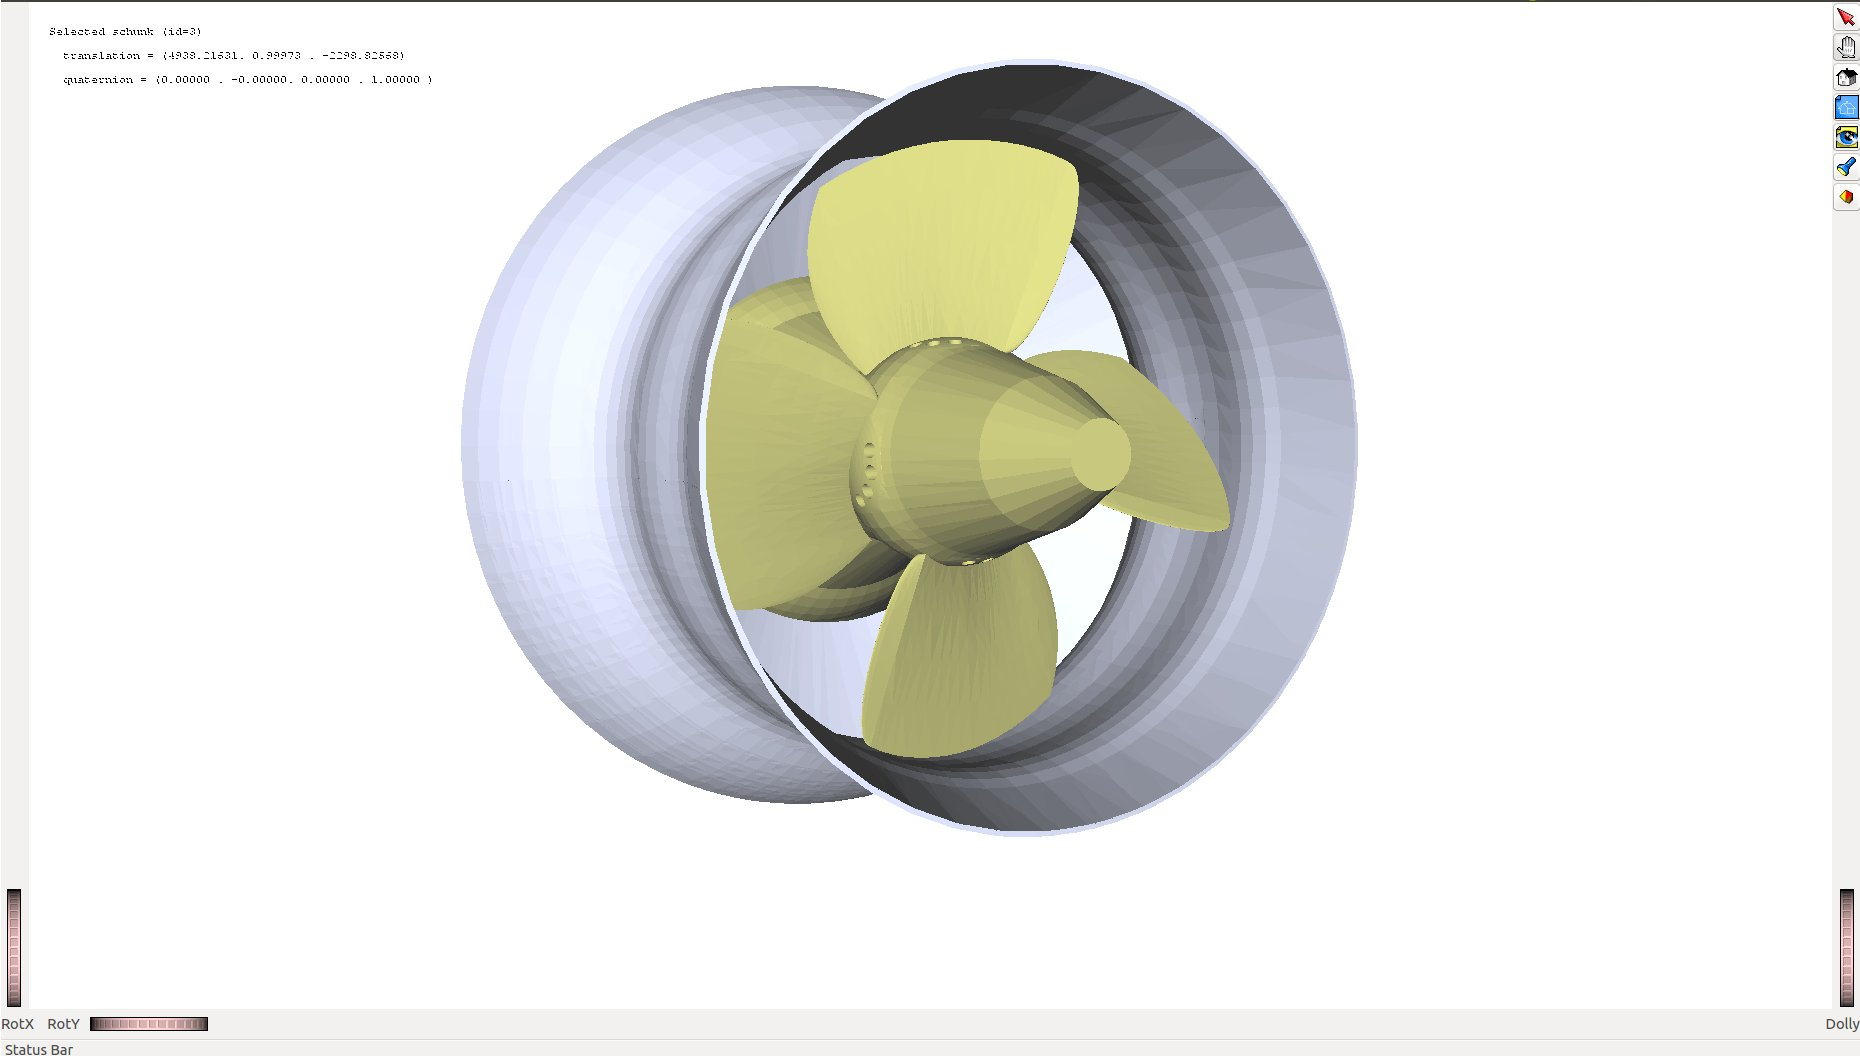
\includegraphics[width=\columnwidth]{figs/openrave/rotor_openrave}
	\caption{Turbina simulada no ambiente do \textit{OpenRAVE}.}
	\label{fig::rotor_openrave}
\end{figure}

Cada manipulador robótico a ser simulado deve ter sua estrutura modelada e suas
juntas assinaladas. Cada elo do robô deve ter sua geometria especificada ou um
modelo deve ser importado de um arquivo externo. A sua posição referente ao eixo
de coordendas da base do manipulador, assim como o eixo de rotação e os ângulos
limites de cada junta devem ser descritos de maneira a formar uma representação
completa do manipulador no ambiente de simulação. Para uma primeira análise,
foram escolhidos dois manipuladores industriais padrão com dimensões dentro de
faixas que representassem um manipulador de médio e grande porte. Como
manipulador de médio porte foi escolhido o modelo \textit{KR 30} do fabricante
\textit{Kuka Robotics} e para o manipulador de grande porte o modelo
\textit{KR 30l16}, do mesmo fabricante, foi selecionado.
A escolha desses manipuladores é justificada, em um primeiro momento, para uma
familiarização com o ambiente de simulação e uma perspectiva das dimensões
necessárias e limites para utilização manipuladores industriais dentro da
turbina.

O manipulador \textit{Kr30} é um manipulador de médio porte, com capacidade de
30kg de carga, 45kg de carga adicional, alcance máximo de 2033mm. A figura
\ref{fig::kukakr30_openrave} ilustra o modelo gerado no ambiente de simulação. 

\begin{figure}[h!]
\centering
	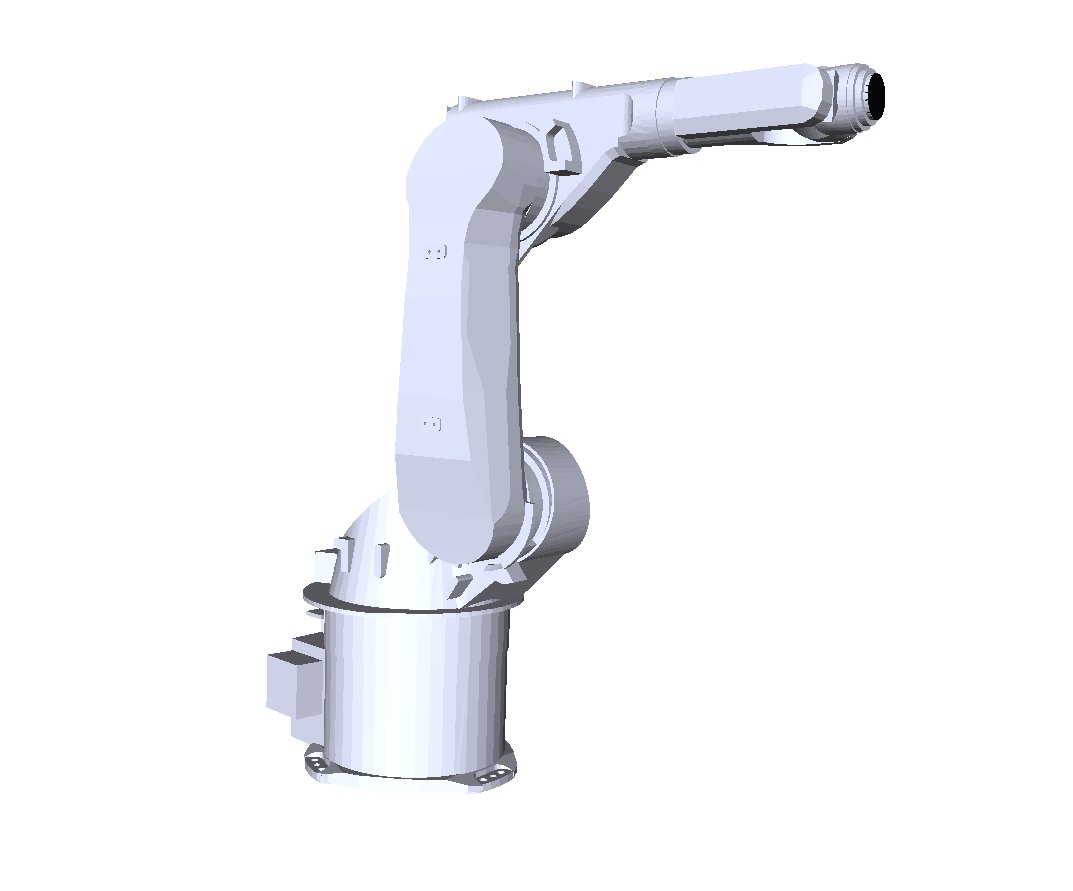
\includegraphics[width=0.8\columnwidth]{figs/openrave/kukakr30_openrave}
	\caption{Manipulador industrial modelo Kuka-KR30 no ambiente de simulação.}
	\label{fig::kukakr30_openrave}
\end{figure}

Por sua vez, o manipulador de grande porte, ilustrado na figura
\ref{fig::kukakr30l16_openrave} é uma versão extendida do manipulador \textit{KR
30} com alcande de 3102mm e carga reduzida para 16kg no efetuador e 45kg de 
carga adicional. Mesmo com a redução de carga o manipulador ainda se
encontra dentro de uma região aceitável, visto que o peso do sistema de
metalização é de 8,5kg.

\begin{figure}[h!]
\centering
	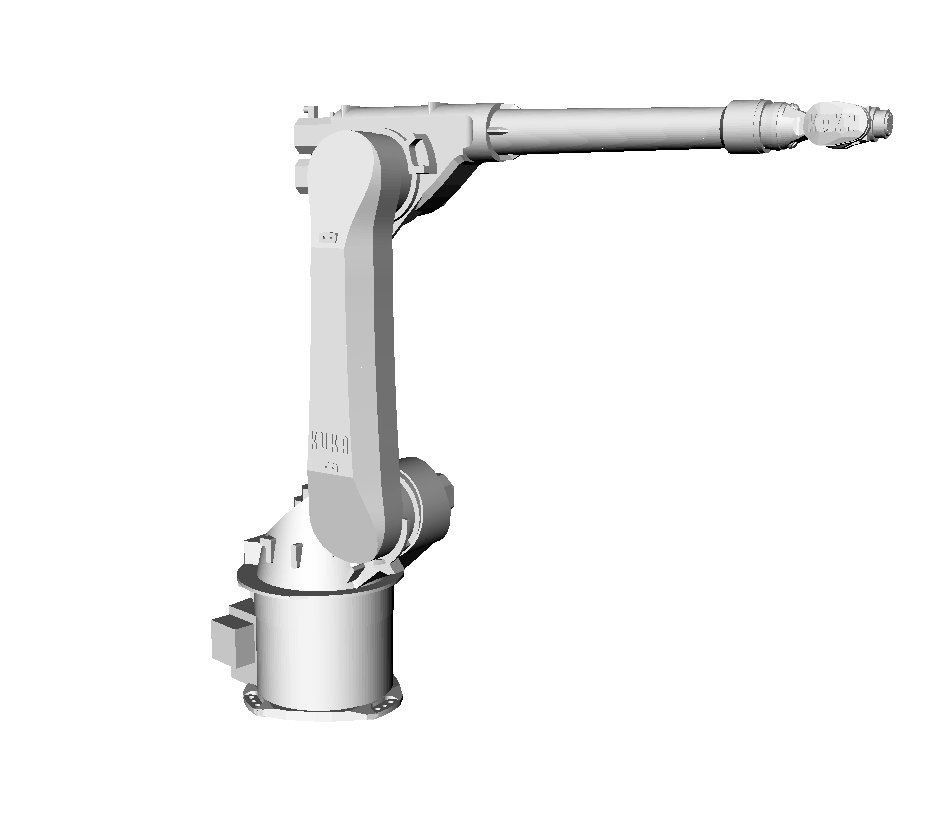
\includegraphics[width=0.8\columnwidth]{figs/openrave/kukakr30l16_openrave}
	\caption{Manipulador industrial modelo Kuka-KR30l16 no ambiente de simulação.}
	\label{fig::kukakr30l16_openrave}
\end{figure}

A especificação do alcance máximo do robô provê apenas a informação do ponto
mais distante de sua base que o manipulador consegue alcançar. Para a descrição
geométrica do espaço de trabalho, é necessário observar cada junta de revolução
ou prismática do robô e, também o tamanho dos elos. A partir dessas informações
é possível gerar um envelope que englobe todo o espaço em que é possível que o
manipulador se posicione. Entretanto, para o contexto da metalização, no qual a
tarefa a ser realizada impõe restrições de posição, orientação e velocidade, é
necessário analisar também a manipulabilidade do manipulador em cada posição.
Utilizando-se o ambiente de simulação do \textit{OpenRAVE} é possível gerar,
numericamente, uma representação visual em 3 dimensões do espaço de trabalho e
também do graus de liberdade em cada ponto do epaço. Esse estudo possibilita,
rapidamente, um entendimento básico do comportamento do robô dentro de seu
espaço de trabalho e, também, proporciona uma maior capacidade de discernimento
do posicionamento da base do robô em relação à turbina para que a seja possível
um melhor aproveitamento do manipulador. A figura \ref{fig::workspace_openrave} ilustra o espaço de
trabalho do manipulador \textit{Kuka KR 30l16}, na qual o robô se
encontra no centro da esfera e cada ponto em que o manipulador consegue
alcançar é representado por uma cor, sendo que quanto mais vermelhor mais graus
de liberdade o efetuador possuí naquela posição.

\begin{figure}[h!]
\centering
	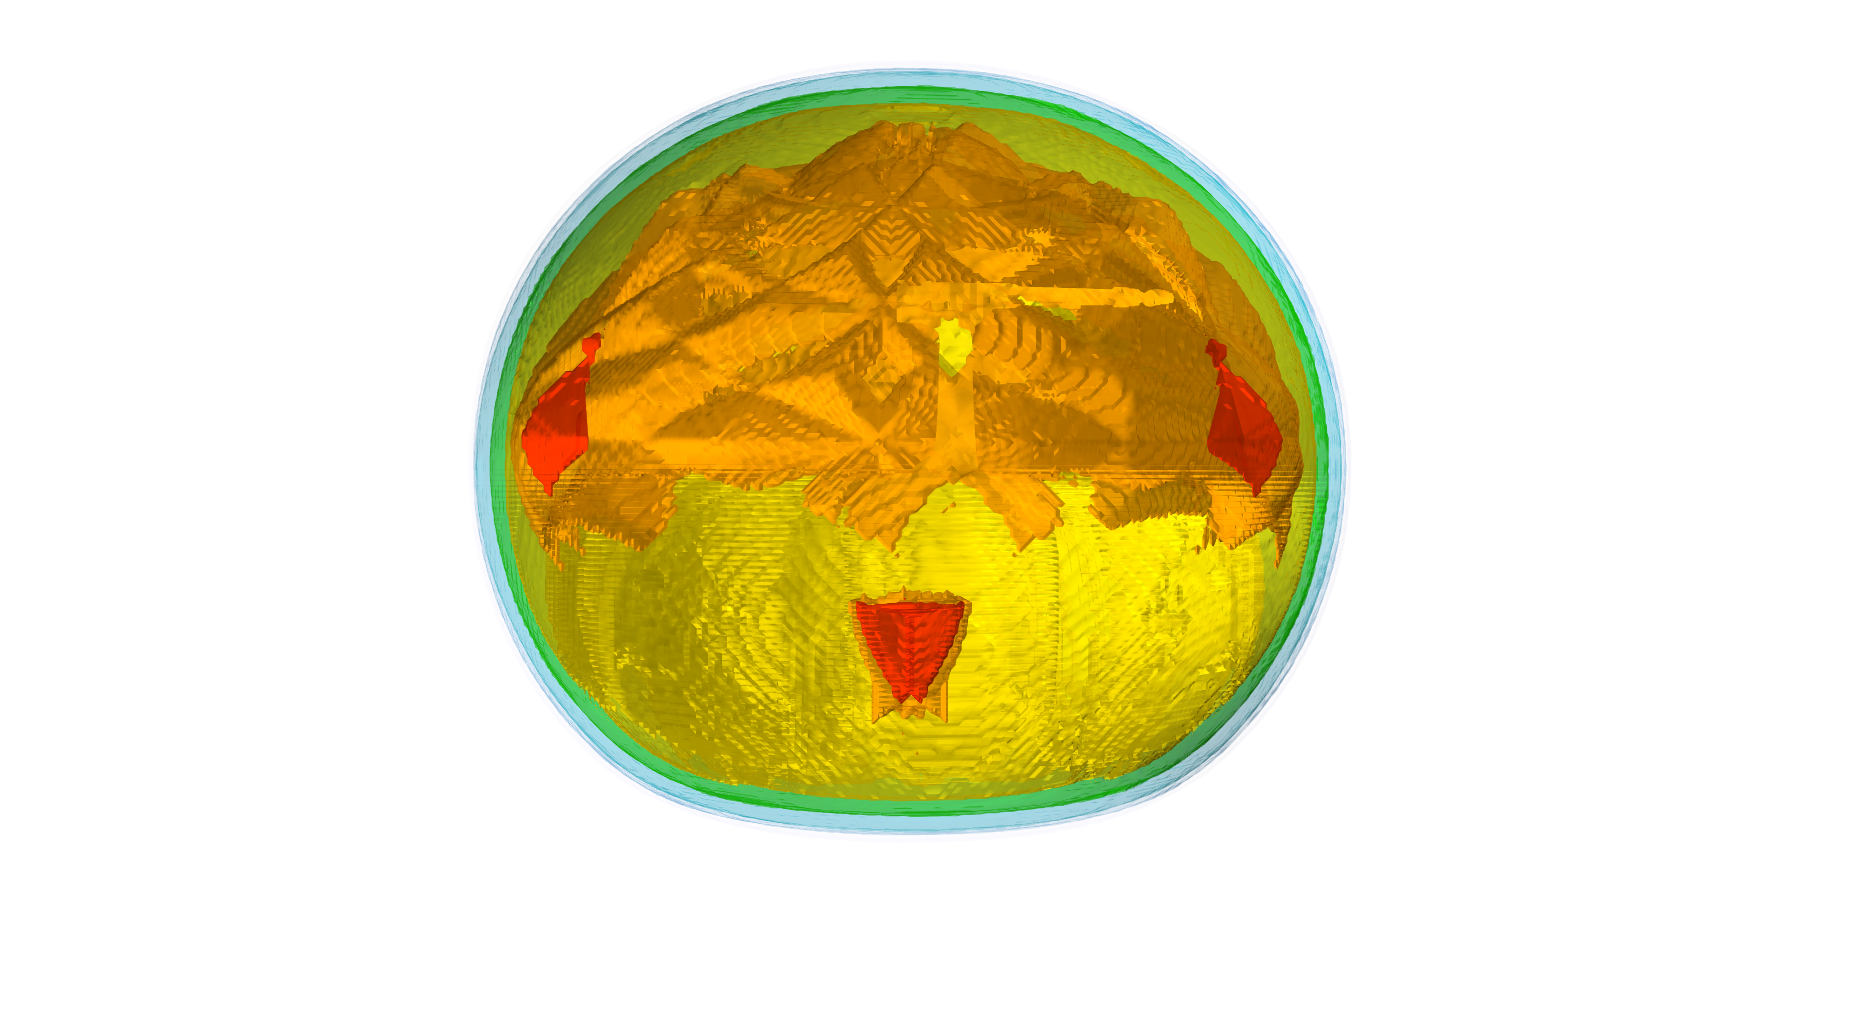
\includegraphics[width=\columnwidth]{figs/openrave/workspace_kr30l16_openrave}
	\caption{Representação do espaço de trabalho do Manipulador industrial
	modelo Kuka-KR30l16.}
	\label{fig::workspace_openrave}
\end{figure}

Uma vez que o ambiente de simulação foi configurado, é possível testar diversos
cenários com os diferentes manipuladores já modelados. Essa característica
possibilita uma análise rápida para validação de conceitos e, também, o teste
de posicionamento de manipuladores com detecção de colisôes. A figura
\ref{fig::position_test_openrave} ilustra a validação de posicionamento do
manipulador \textit{Kuka KR 30} para um ponto extremo da pá. 

\begin{figure}[h!]
\centering
	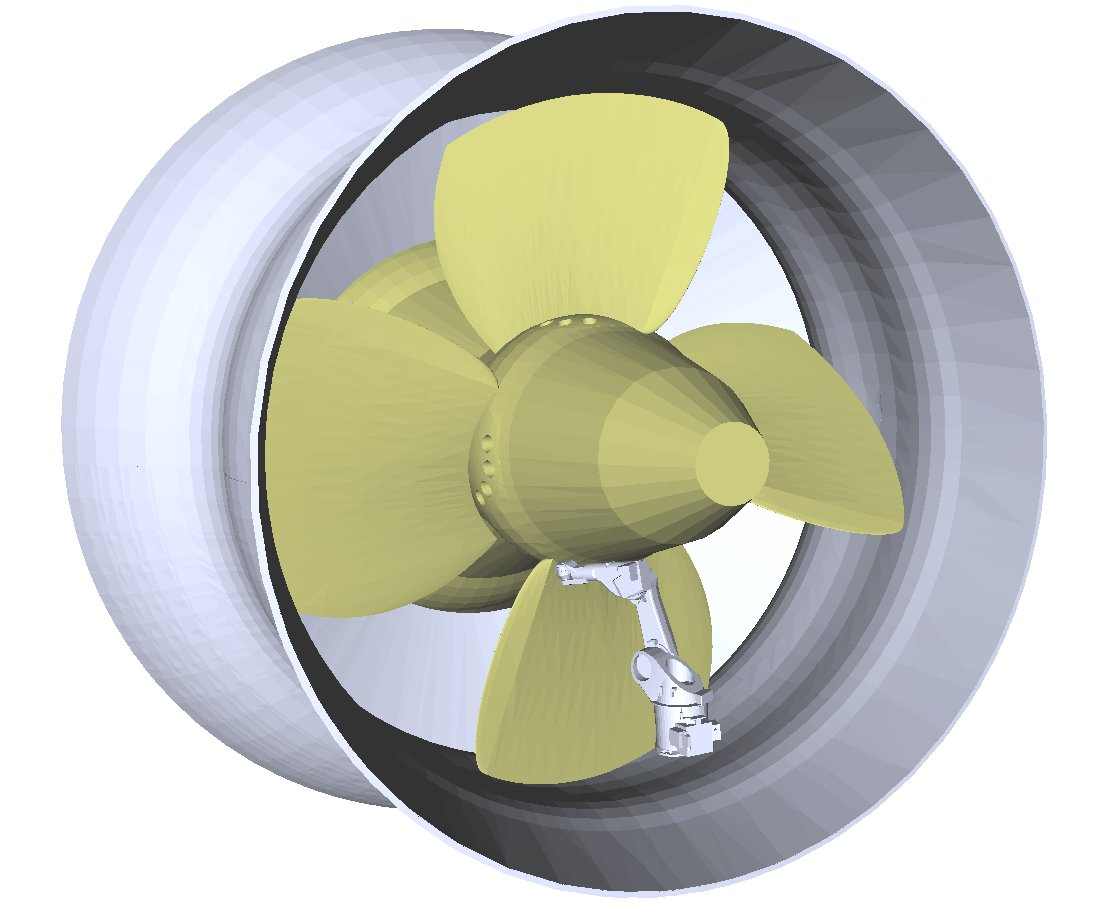
\includegraphics[width=\columnwidth]{figs/openrave/position_test_openrave}
	\caption{Representação do espaço de trabalho do Manipulador industrial
	modelo Kuka-KR30l16.}
	\label{fig::workspace_openrave}
\end{figure}

Após uma primeira análise, verificou-se uma dificuldade de posicionamento do
modelo \textit{Kuka KR 30} de maneira que fosse possível a metalização completa
de uma face da pá do rotor sem a necessidade de movimentação da base. Por outro
lado, a utilização de uma manipulador de grande porte, como o \textit{Kuka KR
30l16}, torna-se muito complexa para o processamento das faces voltadas para a
Jusante, pois o espaço confinado entre as pás dificulta a movimentação do
manipulador. \textbf{O referencial zero para o ângulo das pás não foi
fornecido e foi utilizado o ângulo de $45^o$ em relação a linha perpendicular ao
fluxo d'água como posição de maior arbertura}. Com as informações geradas até o
momento, não é possível descartar a viabilidade técnica de nenhuma das soluções
e um estudo mais detalhado do posicionamento ótimo da base do manipulador deverá
ser realizado. Esse estudo mais detalhado possibilitará confirmar a viabilidade
das soulções e, caso positivo, a definição do o menor número de movimentações
para um manipulador de médio porte e a verificação de uma posição viável para
 o processamento completo da parte à Jusante da pá utilizando-se um manipulador de
grande porte.
